\subsection{Architektur}
\label{subsec:kubernetes:architecture}
% TODO: how to cite everything from kubernetes docs?
Die Architektur von Kubernetes besteht aus Rechnern, welche zu einem Cluster zusammengeschlossen werden.
Hierbei besteht das Cluster aus einer oder mehreren \textbf{Worker machines}, welche in Kubernetes \emph{Knoten}
genannt werden. Diese Knoten sind dafür zuständig die eigentliche Last, die \textbf{Pods}, zu betreiben.
Die Kontrollebene\footnote{Containerorchestrationsschicht, welche die API zum Definieren, Bereitstellen und Verwalten von Containern bereitstellt}
ist verantworlich für die Verwaltung von Knoten und Pods innerhalb des Clusters. 
Um Fehlertoleranz und eine hohe Verfügbarkeit zu gewährleisten, besitzt ein Kubernetes Cluster mehrere Knoten und
die Kontrollebene läuft verteilt über mehrere Systeme \cite{kubernetesComponents}. 

\begin{figure}
  \centering
  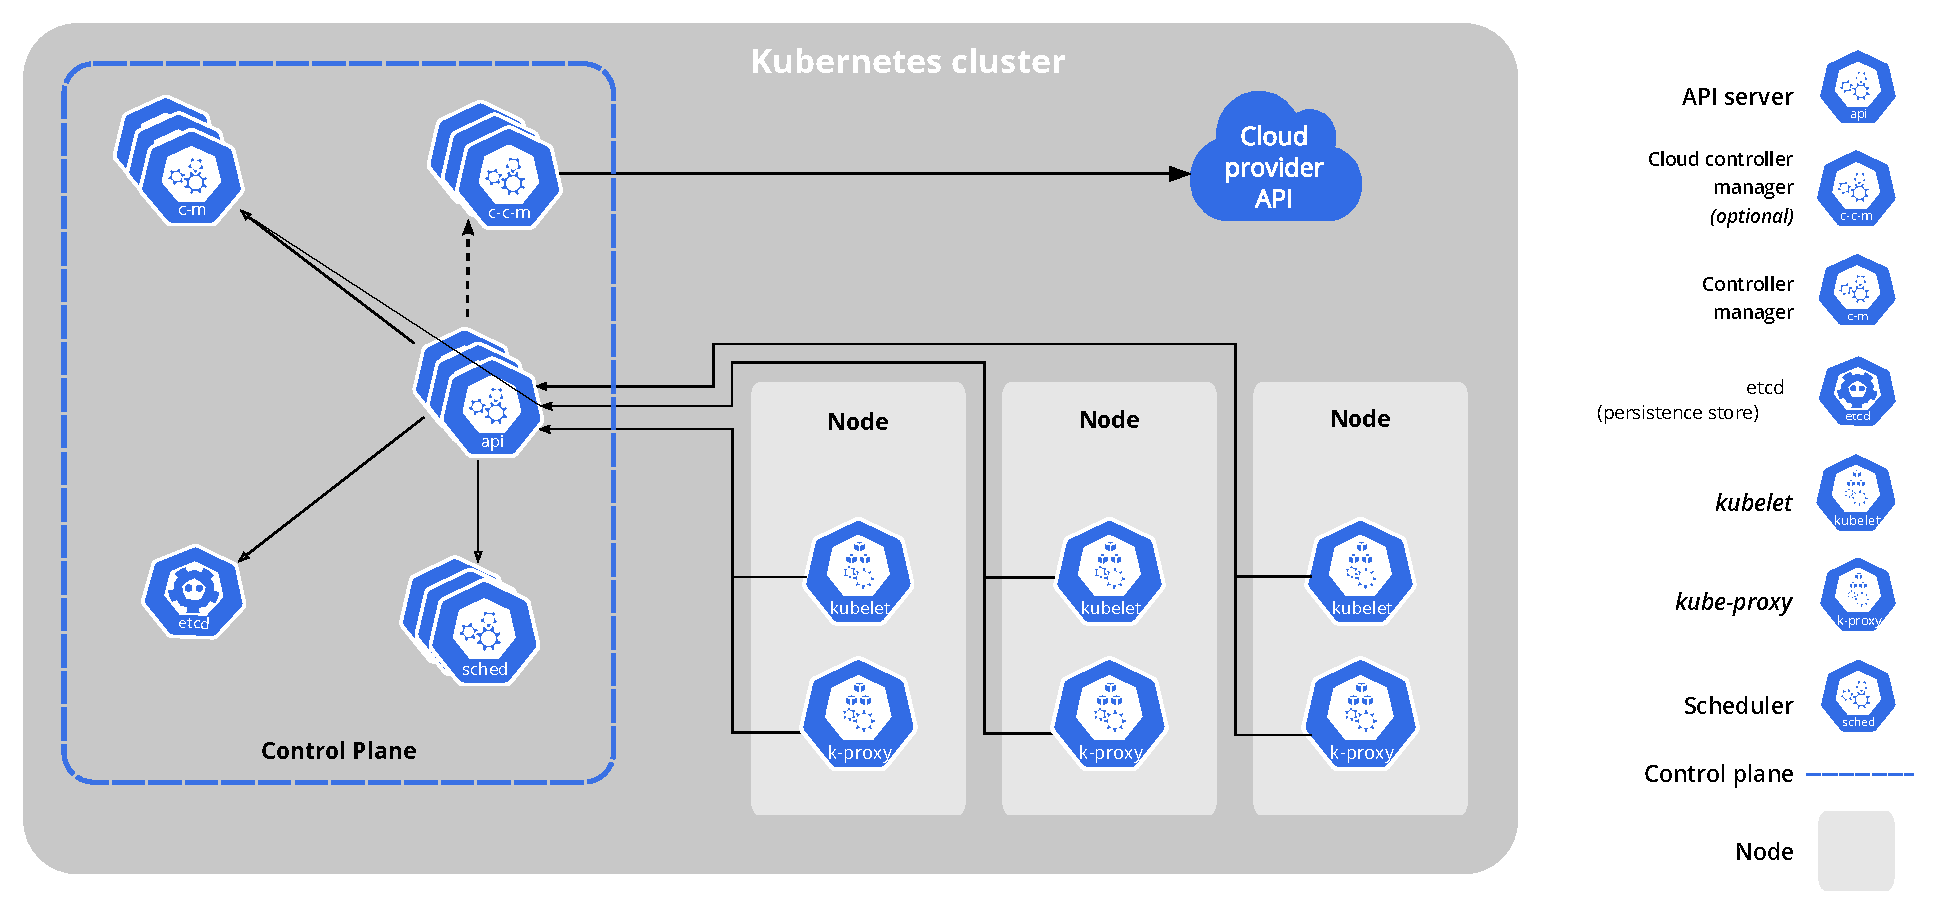
\includegraphics[width=1.2\textwidth]{gfx/chapters/2_grundlagen/components-of-kubernetes.pdf}
  \caption{Architektur eines Kubernetes Clusters}
  \source{\cite{kubernetesComponents}}
  \label{fig:kubernetes_architecture}
\end{figure}

In \ref{fig:kubernetes_architecture} werden die einzelnen Komponenten eines Kubernetes Clusters dargestellt.
Die Kontrollebene besteht dabei aus den folgenden Teilen:
\begin{itemize}
  \item etcd
  \item kube-scheduler
  \item kube-apiserver
  \item kube-controller-manager
\end{itemize}

\paragraph{Etcd} dient als Key-Value Speicher für jegliche Cluster Daten.
Der API-Server ist hierbei die einzige Komponente im Cluster, welche direkt mit dem verteilten Speichersytem interagiert \cite{Hausenblas2019}.

\paragraph{Kube-Scheduler} wird im Cluster eingesetzt, um neu erstellte Pods einem Knoten zuzuweisen.
Hierbei werden Werte wie Ressourcenanforderungen, Hardware, Software oder Richtlinien Beschränkungen 
als Faktoren für die Zuweisung verwendet \cite{kubernetesComponents}.

\paragraph{Kube-apiserver} ist der Einstiegspunkt und die zentrale Managmenteinheit des Cluster \cite{Hausenblas2019}. 
Alle Anfragen an das Cluster werden über den API-Server verarbeitet.
Strukturiert ist der API-Server mithilfe einer REST-HTTP API, welche JSON Daten für Anfragen außerhalb des Clusters
oder Protobuf\footnote{Protobuf ist Googles sprach- und plattformneutraler, erweiterbare Mechanismus zur Serialisierung strukturierter Daten \cite{protobuf}.}
bei der Kommunikation innerhalb des Clusters verwendet \cite{Hausenblas2019}.

\paragraph{Kube-controller-manager} verwaltet Controller innerhalb des Clusters.
Jedem Objekt wird dabei ein eigener Controller zugewiesen.

% TODO: newLine 
\vspace{5mm}
Standardmäßig werden Kontrollebenenkomponenten und Knotenkomponenten auf unterschiedlichen Maschinen ausgeführt,
was nicht zwingend notwendig ist, jedoch zur Hochverfügbarkeit und Ausfallsicherheit beiträgt \cite{kubernetesComponents}. 
Jeder Knoten, der dem Cluster angeschlossen ist, besitzt folgende Komponenten:
\begin{itemize}
  \item Kubelet
  \item Kube-Proxy
  \item Containerlaufzeitumgebung
\end{itemize}

\paragraph{Kubelet} wird als \emph{Agent} auf jedem Knoten im Cluster ausgeführt. 
Es registiert den Knoten am Cluster und ist für die Bereitstellung der Pods zuständig.
Kubelet ist ausschließlich für Container zuständig, die von Kubernetes erstellt wurden \cite{kubernetesComponents}.

\paragraph{Kube-Proxy} ist ein Netzwerk Proxy, der für die Implementierung des Service Konzepts \ref{subsec:kubernetes:service}
zuständig ist. 
Dabei wird sichergestellt, dass die Kommunikation von Pods innerhalb und außerhalb des Clusters möglich ist.

\paragraph{Containerlaufzeitumgebung} betreibt die von Kubelet angeforderten Container für einen Pod. 
Jede Containerlaufzeitumgebung muss das 
\ac{CRI}\footnote{Eine Spezifikation von APIs für Containerlaufzeitumgebungen, um mit Kubelet zu interagieren \cite{cri}.} implementieren.
